\section{Boosting}
% Approach and results with respect to the Boosting approach
\subsection{Hyper-parameter Tuning}
AdaBoost was chosen as our boosting algorithm. The weak classifiers used were decision trees. Hyper-parameter tuning was done using grid search over the parameters \verb|max_depth|, which controls the maximum depth of the trees used as weak classifiers, and \verb|num_classifiers| which controls the total number of trees used. The range searched for \verb|num_classifiers| was $[50, 100, 200, 500]$ and the range of \verb|max_depth| was $[2, 5, 10, 25]$. It was only possible to search a small range of parameters because grid search scales in $O(n*m)$ time where $n$ and $m$ are the numbers of candidates for each hyper-parameter, and because training the model can take a long time, especially when using many deep trees. The performance of each model in the search space was assessed using 5-fold cross validation and the model with the best average accuracy was chosen as our final model. \autoref{fig:BoostTuning} shows the results of the grid search. There seems to be only a small different in model accuracy between models with different hyper-parameters. The final hyper-parameters chosen were \verb|num_classifiers = 100| and \verb|max_depth = 2|. This is because they achieved the best cross-validated accuracy. 

\begin{figure}
    \centering
    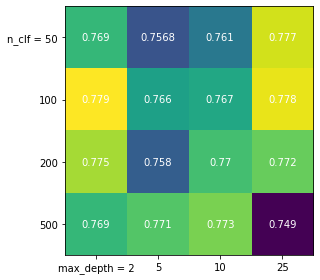
\includegraphics[width= 0.4\textwidth]{figures/hyperparam_tuning_boosting.png}
    \caption{Hyper-parameter grid search for AdaBoost classifier}
    \label{fig:BoostTuning}
\end{figure}

\subsection{Analysis of misclassification}
The model achieved approximately 77\% accuracy on the test data. It had a false positive rate of 0.17 and a false negative rate of 0.29 suggesting that negative reviews are more likely to be misclassified. \autoref{fig:MisclassLengths} shows a histogram of the lengths of misclassified and correctly classified reviews. There seems to be no significant effect of review length on classification quality. This is perhaps surprising given the embedding model is optimised for shorter sentences and suggests that the 'folding' strategy employed in data processing is sufficient to retain the majority of the sentiment information present in the longer reviews.

Qualitatively, the reviews that were misclassified often contained many negative individual words but conveyed a positive point overall, for example this excerpt from a review which was misclassified as negative: "I blamed this very unusual voting pattern (a sudden surge in 1 ratings, with a high 10 rating, dropping only gradually and then suddenly reversing course and jumping at the 1 rating level) on only one thing: hatred for Leonardo DiCaprio. Believe me, I\'ve tuned into enough chat rooms to see the banter by young people (young men, mostly), who defame him left and right. They absolutely hate the man,..." This sentence clearly has a negative sentiment but the sentiment is not about the film, rather about a tangential issue which the author is using to illustrate their point in defence of the film.

Similarly this excerpt from another review which was misclassified as negative: " What results is a relentlessly chilling experience that feels very real and very disturbing, despite the fact that the story itself is fake." This is a negative sentiment but in the context of the film - in the horror genre - it is a good thing. It is easy to see why the model would misclassify these examples without knowledge of the context surrounding them.

\begin{figure}
    \centering
    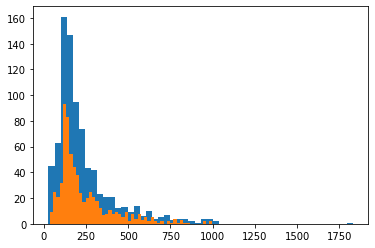
\includegraphics[width= 0.6\textwidth]{figures/Misclass_Lenghts.png}
    \caption{Lengths of correctly classified (blue) and misclassified (red) reviews.}
    \label{fig:MisclassLengths}
\end{figure}